\documentclass{beamer}
%
% Choose how your presentation looks.
%
% For more themes, color themes and font themes, see:
% http://deic.uab.es/~iblanes/beamer_gallery/index_by_theme.html
%
\mode<presentation>
{
  \usetheme{Boadilla}      % or try Darmstadt, Madrid, Warsaw, ...
  \usecolortheme{beaver} % or try albatross, beaver, crane, ...
  \usefonttheme{default}  % or try serif, structurebold, ...
  \setbeamertemplate{navigation symbols}{}
  \setbeamertemplate{caption}[numbered]
  
} 

\usepackage{xcolor,colortbl}
\usepackage[english]{babel}
\usepackage[utf8x]{inputenc}
\usepackage{courier}
\usepackage{dsfont}
\usepackage{verbatim} 
\usepackage{enumerate}
\usepackage{tikz}
\usepackage{multirow}
\usepackage{venndiagram}
\usepackage{epigraph} 
%\usepackage{xcolor}
\usepackage{makecell}

%\usepackage{enumitem}

\usepackage{hyperref}
\hypersetup{
    colorlinks=true,
    linkcolor=blue,
    filecolor=magenta,      
    urlcolor=cyan,
}

% R stuff!
\usepackage{listings}
\definecolor{codegreen}{rgb}{0,0.6,0}
\definecolor{codegray}{rgb}{0.5,0.5,0.5}
\definecolor{codepurple}{rgb}{0.58,0,0.82}
\definecolor{backcolour}{rgb}{0.95,0.95,0.92}

\lstdefinestyle{mystyle}{
    backgroundcolor=\color{backcolour},    
    commentstyle=\color{codegreen},
    keywordstyle=\color{black},
    numberstyle=\tiny\color{codegray},
    stringstyle=\color{codepurple},
    basicstyle=\ttfamily\footnotesize,
    breakatwhitespace=false,         
    breaklines=true,                 
    captionpos=b,                    
    keepspaces=true,                 
    numbers=left,                    
    numbersep=5pt,                  
    showspaces=false,                
    showstringspaces=false,
    showtabs=false,                  
    tabsize=2
}

\lstset{style=mystyle}


\setbeamertemplate{enumerate items}[default]
\setbeamertemplate{itemize item}[triangle]

%\setitemize{label=\usebeamerfont*{itemize item}%
%  \usebeamercolor[fg]{itemize item}
%  \usebeamertemplate{itemize item}}



\title[Introduction to Statistics]{Elections and Polling Methods}
\subtitle{How are polls carried out?}
\author{Grinnell College}
\date{}

\graphicspath{{img/}}

\begin{document}

\begin{frame}
  \titlepage
\end{frame}

\begin{frame}
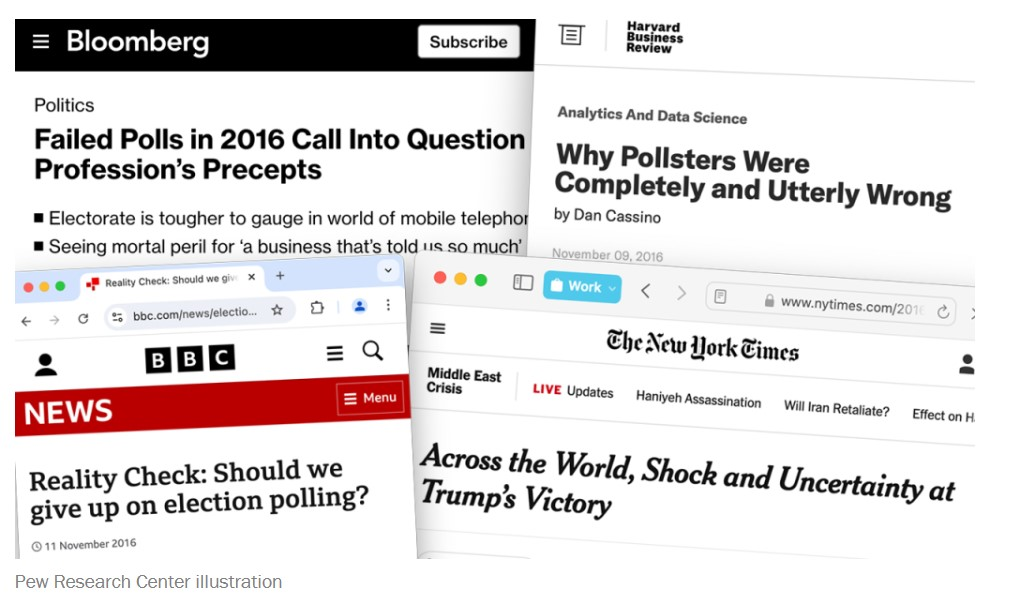
\includegraphics[scale=.7]{img/polling_headlines.jpg}    
\end{frame}

\begin{frame}{Polling Outline}
Polling is \textbf{complicated} \vspace{8mm}

These are a summary of some important things about polling mixed in with ideas we have seen covered in class already. \vspace{8mm}

Most of the new stuff I am taking from articles published by:
\begin{itemize}
    \item Pew Research Center
    \item FiveThirtyEight.com
\end{itemize}
\end{frame}

\begin{frame}{Background}
How US elections work (extremely simplified): \vspace{4mm}

Every 4 years there is a presidential election
\begin{itemize}
    \item president and VP are elected
    \item some senate seats are elected (\# varies)
    \item all house seats are elected (438 total)
    \item many other positions at the state level are elected
\end{itemize} \vspace{4mm}

Every 2 years (between presidential elections)
\begin{itemize}
    \item some senate seats are elected (\# varies)
    \item all house seats are elected (438 total)
    \item many other positions at the state level are elected
    \item frequently called 'mid-term' elections
\end{itemize} \vspace{4mm}

Sometimes there are also amendments to state laws that are voted on too.


\end{frame}

\begin{frame}{Background}
In 2016 and 2020, polling did not do a very good job (in many people's opinions) of predicting the presidential election results. \vspace{10mm}

In both years, polls underestimated the strength of Republican candidates. \vspace{10mm}

Polls generally performed better in the mid-term elections in 2018 and 2022.
\end{frame}

\begin{frame}{Big Things in Polling}
In my opinion, there are really 2 big areas of concern in polling. But there is much that goes into each. \vspace{4mm}

\begin{enumerate}
    \item Sample Selection (hard)
    \begin{itemize}
        \item How do we pick people
        \item Representative?
    \end{itemize}
    \vspace{6mm}
    \item Estimation (easy)
    \begin{itemize}
        \item confidence intervals
        \item frequent use of the term Margin of Error (ME)
    \end{itemize}
\end{enumerate}
\end{frame}

\begin{frame}{Review -- The Statistical Framework}
\begin{center}
\usetikzlibrary{decorations.pathreplacing,positioning, arrows, shapes, calc,shapes.multipart}
\tikzstyle{block1} = [rectangle, draw, fill=yellow!20, 
    text width=10em, text centered, rounded corners, minimum height=6em]
\tikzstyle{block2} = [rectangle, draw, fill=yellow!20, 
    text width=5em, text centered, rounded corners, minimum height=3em]
\tikzset{
    %Define standard arrow tip
    >=stealth,
    % Define arrow style
    pil/.style={
           ->,
           thick,
           shorten <=2pt,
           shorten >=2pt,}
}
\tikzstyle{line} = [draw, -latex]
\begin{tikzpicture}[node distance = 3cm, auto]
            % Place nodes
            \node [block1] (pop) {Population \\ (Parameter)};
            \node [block2, below of=pop] (samp) {Sample \\ (Statistic)};
            
            % Draw edges
            \draw[<-, >=latex, shorten >=2pt, shorten <=2pt, bend right=45, thick]  (pop.west) to node[auto, swap] {Inference}(samp.west);
            \draw[<-, >=latex, shorten >=2pt, shorten <=2pt, bend right=45, thick] (samp.east) to node[auto, swap] {Study Design}(pop.east); 
            
        \end{tikzpicture}
  \end{center}
\begin{itemize}
    \item almost always the parameter and statistic of interest in polls is a proportion (p) or difference in proportions ($p_1 - p_2$)
    \item we can use confidence interval stuff we covered to estimate these
\end{itemize} 
\end{frame}

\begin{frame}{Review -- Sample Selection}
How do we select people? \vspace{6mm}

We want our sample to be \textbf{representative} of our population.
\begin{itemize}
    \item this means that our sample is nearly the same as our population, only smaller
        \begin{itemize}
            \item i.e.: same proportions M/F, same age/ethnic demographics
        \end{itemize} \vspace{4mm}
    \item a representative sample allows us to generalize our results from the sample to the pop.
\end{itemize}
\end{frame}

\begin{frame}{Review -- How do we select people?}
\textbf{Random Sample}

We can choose people at random from our population to reduce the chances of getting a biased sample.
\begin{itemize}
    \item usually the best way to get a representative sample
    \item allows us to \textbf{generalize} from our sample to the pop.
\end{itemize} \vspace{8mm}

\textbf{Sample Size (n = ?)}
\begin{itemize}
    \item number of people we survey is important (more people = more info)
    \item sample size is very important, but proportion of pop. surveyed is not
    \item affects ME's and CI's we've seen before
    \item you can get good results using a sample of 1000 people for a pop. of 300million
\end{itemize}
\end{frame}

\begin{frame}{Review -- Sampling Frame}
\textbf{Sampling Frame} -- List of people we have access to sample from.
\begin{itemize}
    \item What happens when certain groups of people aren't fully representative in the sampling frame?
\end{itemize}
\end{frame}

\begin{frame}{Review -- Intended vs. Actual population}
\begin{center}
    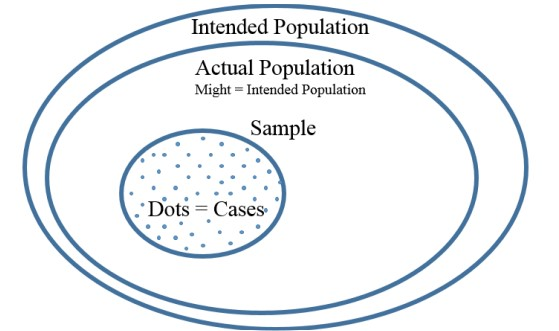
\includegraphics[]{img/actual_intended_pop.jpg}
\end{center}
\text{\tiny source: Dr. Ziegler's Stat 104 notes (ISU)}
\end{frame}

\begin{frame}{Poll Accuracy}
\begin{center}
    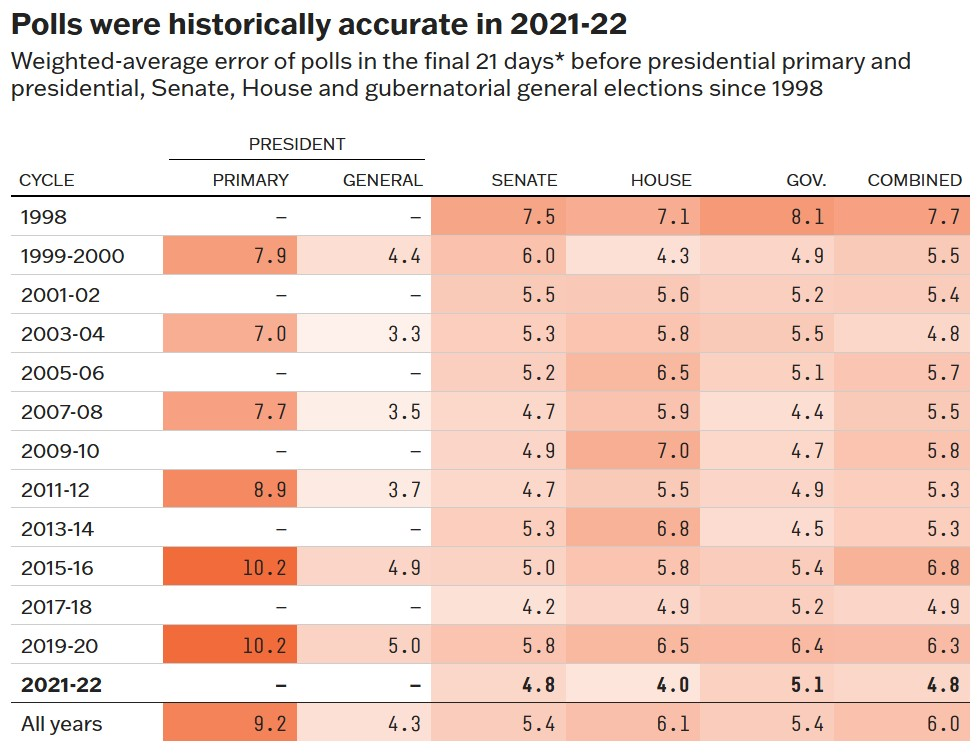
\includegraphics[scale=.55]{img/538_accurate_polling.jpg}
\end{center}
\footnotesize Source: FiveThirtyEight.com
\end{frame}

\begin{frame}{Changes to the Polling Scene}
"...[the] number of active polling organizations has grown significantly, indicating that there are fewer barriers to entry into the polling field. The number of organizations that conduct national election polls more than doubled between 2000 and 2022."
\begin{itemize}
    \item issues? (more on this later too)
\end{itemize}\vspace{6mm}

"This growth has been driven largely by pollsters using inexpensive opt-in sampling methods. But previous Pew Research Center analyses have demonstrated how surveys that use [non-random] sampling may have errors twice as large, on average, as those that use [random] sampling."
\end{frame}

\begin{frame}{Polling Methods}
How have surveys been conducted mostly until the last few years?
\begin{itemize}
    \item land-line phone surveys
    \item cell-phone surveys
    \item internet
    \item emails
    \item 'snail' mail
\end{itemize}
\end{frame}

\begin{frame}{Polling Methods}
\begin{center}
    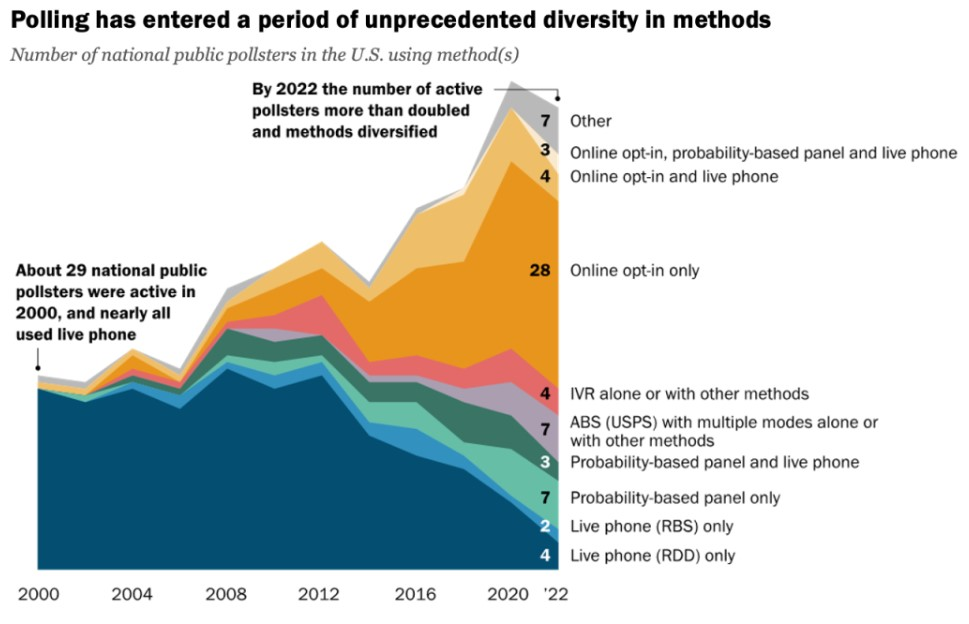
\includegraphics[scale=.7]{img/polling_methods.jpg}
\end{center}    
\end{frame}

\begin{frame}{Changes to the Polling Scene}
"... many of the more prominent polling organizations that use [random] sampling – including Pew Research Center – have shifted from conducting polls primarily by telephone to using online methods, or some combination of online, mail and telephone. The result is that polling methodologies are far more diverse now than in the past."
\end{frame}

\begin{frame}{Margin of Error}
The Margin of Error was used in CI's to quantify uncertainty in our estimation, but...

\begin{center}
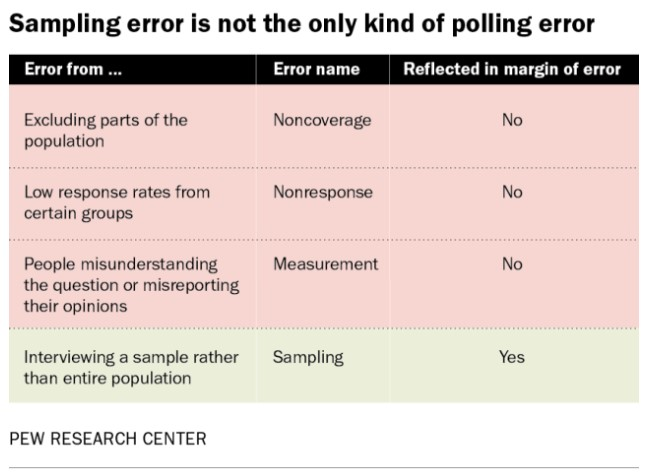
\includegraphics[scale=.8]{img/sampling_error_chart.jpg}
\end{center}
\end{frame}

\begin{frame}{Selecting People for Surveys}
\textbf{MAJOR} issues we've seen
\begin{itemize}
    \item under-representation in samples
    \item non-response bias
\end{itemize} \vspace{10mm}

How do we account for these and get accurate results?
\end{frame}



\begin{frame}{Survey Weighting}
\textbf{Weighting} is a term for adjusting our survey sample so that it is more representative of the population.
\begin{itemize}
    \item we give more 'weight' to groups that are under-represented
    \item idea is to even out the fact that there are less people in this group than we should have in the sample
\end{itemize} \vspace{6mm}

"Historically, public opinion researchers have adjusted their data using a core set of demographic variables to correct imbalances between the survey sample and the population."
\end{frame}

\begin{frame}{Survey Weighting}
Common demographic adjustments
\begin{itemize}
    \item Age
    \item Race/Ethnicity
    \item Sex/Gender
    \item Education
\end{itemize} \vspace{5mm}

"But there is a growing realization among survey researchers that weighting a poll on just a few variables like age, race and gender is insufficient for getting accurate results. Some groups of people – such as older adults and college graduates – are more likely to take surveys, which can lead to errors that are too sizable for a simple three- or four-variable adjustment to work well." 
\end{frame}

\begin{frame}{Survey Weighting}
\begin{center}
    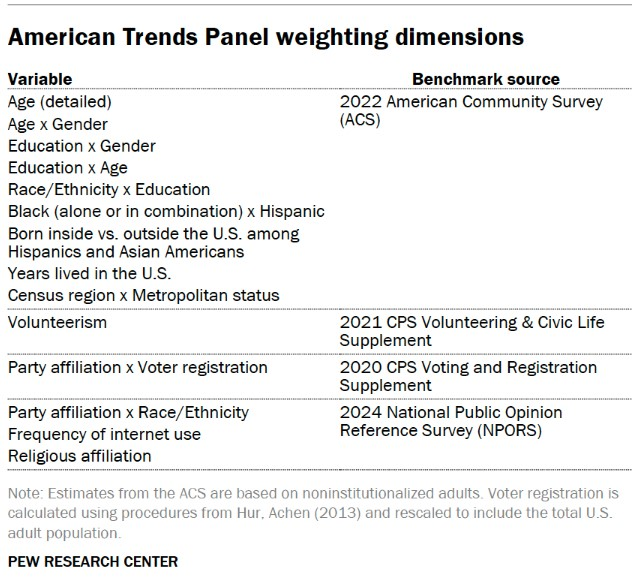
\includegraphics[scale=.75]{img/survey_weighting_variables.jpg}
\end{center} 
\end{frame}

\begin{frame}{Who Shows up to Vote?}
"Predicting who will vote is critical – and difficult. Preelection polls face one crucial challenge that routine opinion polls do not: determining who of the people surveyed will actually cast a ballot." \vspace{8mm}

None of the polling matters if those who show up to vote are different than the group we surveyed.
\begin{itemize}
    \item pollsters make their own educated guesses about turnout
    \item based on historical data
    \item based on measures of voter enthusiasm
    \item EXTREMELY hard to get this right
\end{itemize}
\end{frame}

\begin{frame}{Poll Timing}
"Public opinion on most issues is remarkably stable, so you don’t necessarily need a recent poll about an issue to get a sense of what people think about it. But dramatic events can and do change public opinion, especially when people are first learning about a new topic. For example, polls this summer saw notable changes in voter attitudes following Joe Biden’s withdrawal from the presidential race." \vspace{6mm}

\begin{itemize}
    \item Polls taken right after an event may not pick up shifts in opinion
    \item Dramatic events can affect voter enthusiasm $\rightarrow$ turnout
    \item opinion and enthusiasm have a complicated relationship $\rightarrow$ makes accurate polling even harder
\end{itemize}
\end{frame}

\begin{frame}
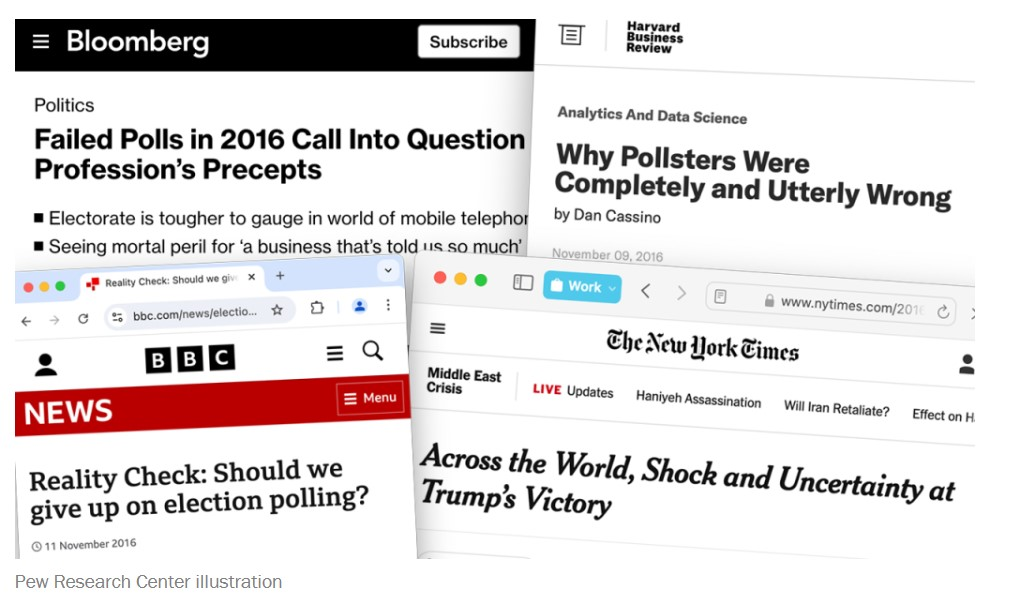
\includegraphics[scale=.7]{img/polling_headlines.jpg}    
\end{frame}

\begin{frame}{Polling Accuracy}
\begin{center}
    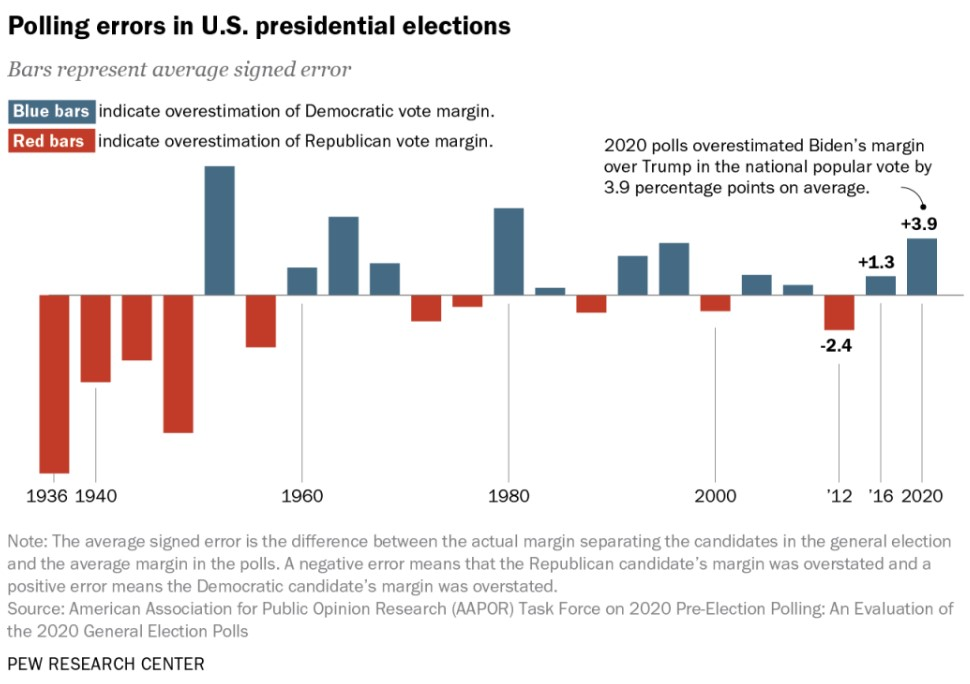
\includegraphics[scale=.7]{img/polling_accuracy.jpg}
\end{center}    
\end{frame}

\begin{frame}{Polling Accuracy}
American Association for Public Opinion Research (AAPOR):

“...the 2020 polls featured polling error of an unusual magnitude: It was the highest in 40 years for the national popular vote and the highest in at least 20 years for state-level estimates of the vote in presidential, senatorial, and gubernatorial contests.”
\end{frame}

\begin{frame}{Frame Title}
PRC: "The 2022 midterms saw generally accurate polling, despite a wave of partisan polls predicting a broad Republican victory. In fact... Moreover, a handful of contrarian polls that predicted a 2022 “red wave” largely washed out when the votes were tallied. In sum, if we focus on polling in the most recent national election, there’s plenty of reason to be encouraged." \vspace{6mm}

FiveThirtyEight: “...polls were more accurate in 2022 than in any cycle since at least 1998, with almost no bias toward either party.”
\end{frame}

\begin{frame}{Sampling Error (again)}
Back to error... people think polls are more accurate than they really are
\begin{center}
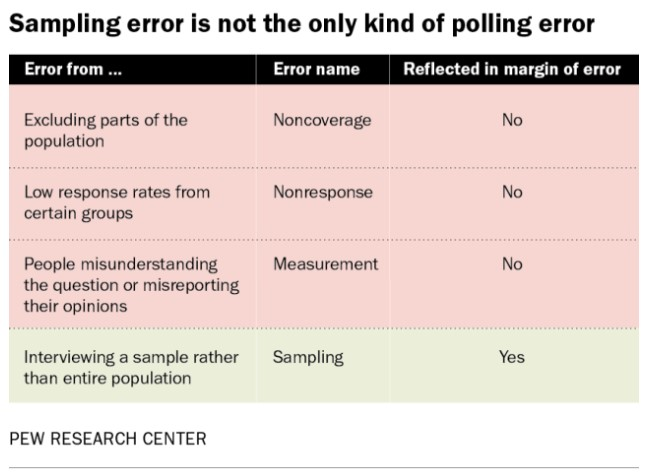
\includegraphics[scale=.8]{img/sampling_error_chart.jpg}
\end{center}
\end{frame}

\begin{frame}{Polling Transparency}
Transparency in how a poll was conducted is associated with better accuracy. \vspace{6mm}

"Participation in these transparency efforts does not guarantee that a poll is rigorous, but it is undoubtedly a positive signal. Transparency in polling means disclosing essential information, including the poll’s sponsor, the data collection firm, where and how participants were selected, modes of interview, field dates, sample size, question wording, and weighting procedures."
\end{frame}

\begin{frame}{Polling Effects on an Election}
Results from polls before an election can influence who turns up to vote. \vspace{8mm}

"Following the 2016 election, many people wondered whether the pervasive forecasts that seemed to all but guarantee a Hillary Clinton victory – two modelers put her chances at 99\% – led some would-be voters to conclude that the race was effectively over and that their vote would not make a difference."
\end{frame}

\begin{frame}{Further Complications}
The presidential election is note determined by national popular vote!
\begin{itemize}
    \item each state has a number of 'electoral votes' = \# senators + \# representatives
    \item for most states whoever wins the state popular vote gets that state's EV's
    \item 538 EVs up for grabs, need 270 to win president race
    \begin{itemize}
        \item barring other legal shenanigans that can throw a wrench into this
    \end{itemize}
\end{itemize}
\end{frame}

\begin{frame}{Sources}
Pew Research Center:
https://www.pewresearch.org/short-reads/2024/08/28/key-things-to-know-about-us-election-polling-in-2024/ \vspace{2mm}

FiveThirtyEight.com
https://fivethirtyeight.com/features/2022-election-polling-accuracy/
\vspace{2mm}

AAPOR:
https://aapor.org/wp-content/uploads/2022/11/AAPOR-Task-Force-on-2020-Pre-Election-Polling\_Report-FNL.pdf
\end{frame}

% \begin{center}
%     \includegraphics[]{}
% \end{center}


%%%%%%%%%%%%%%%%

%\begin{frame}
%\begin{columns}
%
%  \begin{column}{0.45\textwidth}
%%
%  \end{column}
%  \begin{column}{0.45\textwidth}
%%
%  \end{column}
%
%\end{columns}
%\end{frame}


\end{document}


